% $Id: board2.tex 9376 2021-08-31 13:12:43Z mskala $

%
% MSK 008 Board 2 build instructions
% Copyright (C) 2017  Matthew Skala
%
% This program is free software: you can redistribute it and/or modify
% it under the terms of the GNU General Public License as published by
% the Free Software Foundation, version 3.
%
% This program is distributed in the hope that it will be useful,
% but WITHOUT ANY WARRANTY; without even the implied warranty of
% MERCHANTABILITY or FITNESS FOR A PARTICULAR PURPOSE.  See the
% GNU General Public License for more details.
%
% You should have received a copy of the GNU General Public License
% along with this program.  If not, see <http://www.gnu.org/licenses/>.
%
% Matthew Skala
% https://northcoastsynthesis.com/
% mskala@northcoastsynthesis.com
%

\chapter{Building Board 2}

The recommended order for building this module is to assemble Board 2, the
one further from the front panel, first.  That will make it easier to get
all the physical positioning right for the components that bridge between
the boards or pass through the panel.

Note that although I'm describing a separate step for each component value,
and that's how I built my prototype so as to have plenty of photo
opportunities, if you are reasonably confident about your skills you may
find it easier to populate all or most of the board (i.e.\ put the
components in place) and then solder them in a single step.  Except where
noted, the order in which you add components does not matter much.

\section{Preliminaries}

Count out the right number of everything according to the bill of materials. 
There is an abbreviated BOM for Board~2, and a few items from Board~1 used
during the assembly of Board~2, in Table~\ref{tab:b2bom}.

\noindent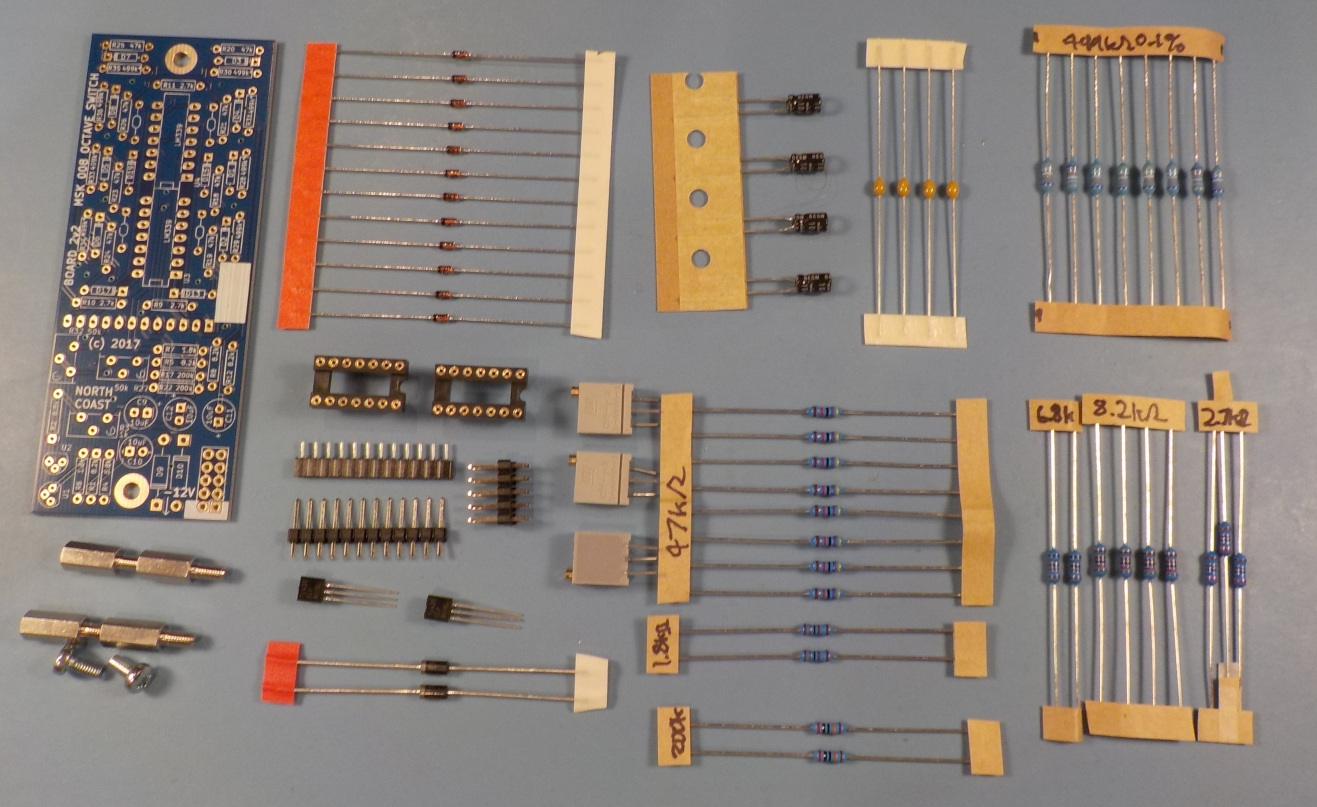
\includegraphics[width=\linewidth]{board2-parts.jpg}

There are three multiturn trimmers to be installed on this board.  Before
installing them, use an ohmmeter to adjust each one to 50\% of its range. 
Measure the resistance along the track, then measure the resistance from the
wiper to one end and adjust to make the wiper half the total track
resistance.  This need not be exact, but having them start near their
midpoints will help with adjustment later,
by reducing issues with interaction among the different settings.  With all
trimmers pre-set to 50\%, the module should basically work even if it is not
at its best, whereas if they are installed at extreme values instead, then
you may have trouble getting it up and running enough to adjust it more
accurately.

\begin{table*}
{\centering
\fbox{This table is not a substitute for the text instructions.}
\vspace{\baselineskip}

\begin{tabular}{rp{1.3in}cp{3in}}
  \textbf{Qty} & \textbf{Ref} & \textbf{Value/Part No.} & \\ \hline
\input{bomdata-2.tex}
\end{tabular}\par}
\caption{Bill of Materials for assembling Board~2.}\label{tab:b2bom}
\end{table*}

Be aware that I sometimes discover trimmers with incorrect printed markings
in incoming parts shipments, in particular trimmers sold to me as
50k$\Omega$ that on testing seem to really be 50k$\Omega$, but the factory
printing says ``10K.'' I think many people who buy trimmers simply feed them
directly into assembly robots without ever reading the printed markings, so
it's easy for this kind of mistake to get into the supply chain.  If you
find a trimmer with unexpected markings in your MSK~008 kit, or if you have
one whose value is in doubt for whatever reason, \emph{test it} with an
ohmmeter and make sure of what it actually is (bearing in mind the tolerance
on track resistance, which may be up to 20\%) before you solder it into a
board.  This centering pre-adjustment step is a good opportunity to do that. 
If you buy a kit from North Coast and verify that it does not contain one
1k$\Omega$ (that is, measured value between 800$\Omega$ and 1200$\Omega$)
and two 50k$\Omega$ trimmers (measured value between 40k$\Omega$ and
60k$\Omega$, regardless of the markings), please contact us for help sorting
the situation out.

\section{Decoupling capacitors}

The four axial ceramic 0.1$\mu$F decoupling capacitors, C1 to C4, are shown on
the board by a special symbol without their reference designators.

\noindent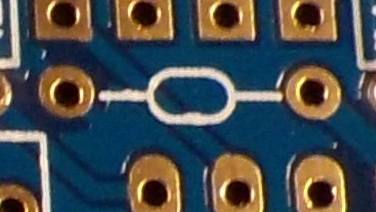
\includegraphics[width=\linewidth]{decoup-symbol.jpg}

Install these four capacitors where the symbol appears.  They are not
polarized and may be installed in either orientation.  These capacitors act
as filters for the power supplies to the comparator chips, preventing any
current spikes associated with their rapid switching from affecting other
things on the same power supply.  An MSK~008 kit should include six of these
capacitors, and only four are used on this board; save the remaining two for
use on Board~1.

\noindent\includegraphics[width=\linewidth]{{cap-0.1u2}.jpg}

\section{Fixed resistors}

Resistors are never polarized.  I like to install mine in a consistent
direction for cosmetic reasons, but this is electrically unnecessary.  In
this module, most resistors are metal film 1\%\ type; a few are 0.1\%\
precision metal film resistors.  Both kinds will usually have blue bodies
and four colour bands designating the value, plus a fifth band for the
tolerance, and these are the resistors shipped in the North Coast
kits.  The tolerance band is brown for 1\%\ and violet for 0.1\%, but note
that we may occasionally ship better-tolerance resistors in the kits than
the specifications require, if we are able to source them at a good price.
Accordingly, I mention only the four value band colours for this type of
resistor; if you are using resistors with other codes, you are responsible
for knowing them.  Note that colour codes on metal film 1\% resistors are
often ambiguous (reading from one end or the other end may give two
different values, both plausible) and some of the colours are hard to
distinguish anyway.  If in doubt, always measure with an ohmmeter before
soldering the resistor in place.

There are no cases in this module of the same nominal resistance value being
used at more than one tolerance, but the 0.1\%\ resistance values are marked
with asterisks (*) on the board silkscreen as a reminder that these
positions require special resistors.

The physical size of the resistors may vary, and details like the exact
colour of the bluish background.  You can see some of that variation in the
photos in these instructions.  Some of the resistance values used in this
module are hard to find, and we source different values from different
suppliers, so not all the resistors in a kit will necessarily be from the
same manufacturer, nor match on non-critical specifications like power
rating and physical size.

\pagebreak

Install the two 1.8k$\Omega$ (brown-grey-black-brown) resistors R6 and R7.
These control the overall current level through the reference voltage
regulators.

\noindent\includegraphics[width=\linewidth]{{res-1.8k}.jpg}

Install the three 2.7k$\Omega$ (red-violet-black-brown) resistors R9, R10,
and R11.  These are part of the divider that generates reference voltages
for the quantizer.

\noindent\includegraphics[width=\linewidth]{{res-2.7k}.jpg}

Install the two 6.8k$\Omega$ (blue-grey-black-brown) resistors R2 and R4. 
These are used in programming the voltage regulators.

\noindent\includegraphics[width=\linewidth]{{res-6.8k}.jpg}

Install the four 8.2k$\Omega$ (grey-red-black-brown) resistors R1, R5, R8,
and R12.  These are used in multiple places in the reference voltage
generator.

\noindent\includegraphics[width=\linewidth]{{res-8.2k}.jpg}

\pagebreak

Install the eight 47k$\Omega$ (yellow-violet-black-red) resistors R18 to R21
and R23 to R26.  These limit the current drawn from the -4.5V reference bus,
inside the quantizers.

\noindent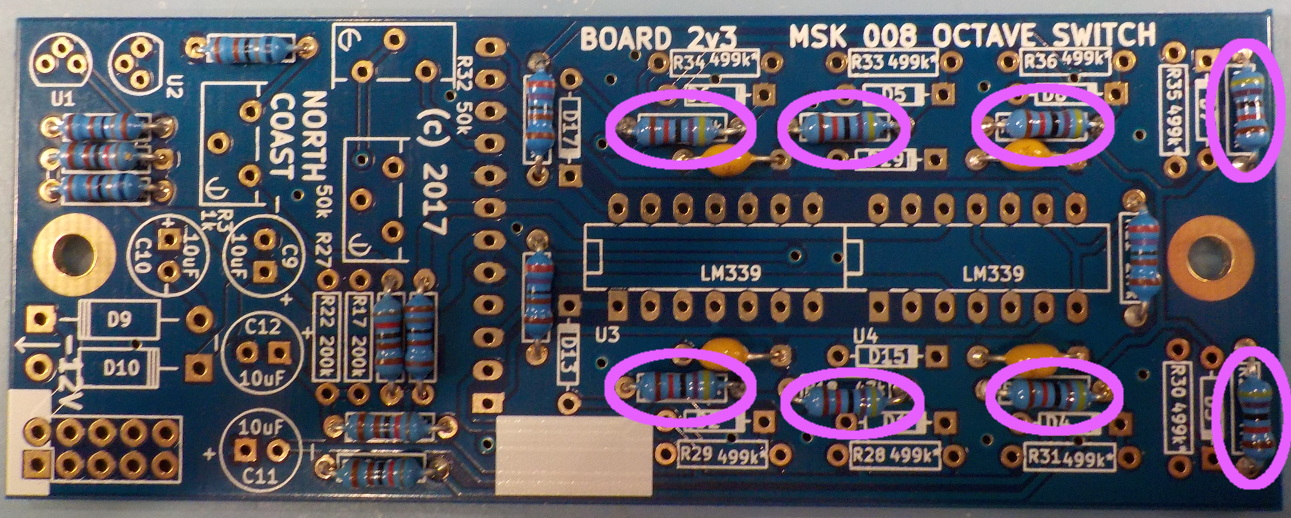
\includegraphics[width=\linewidth]{res-47k.jpg}

Install the two 200k$\Omega$ (red-black-black-orange) resistors R17 and R22. 
These (along with the 50k$\Omega$ trimmers) control the offset of the
quantizer outputs.

\noindent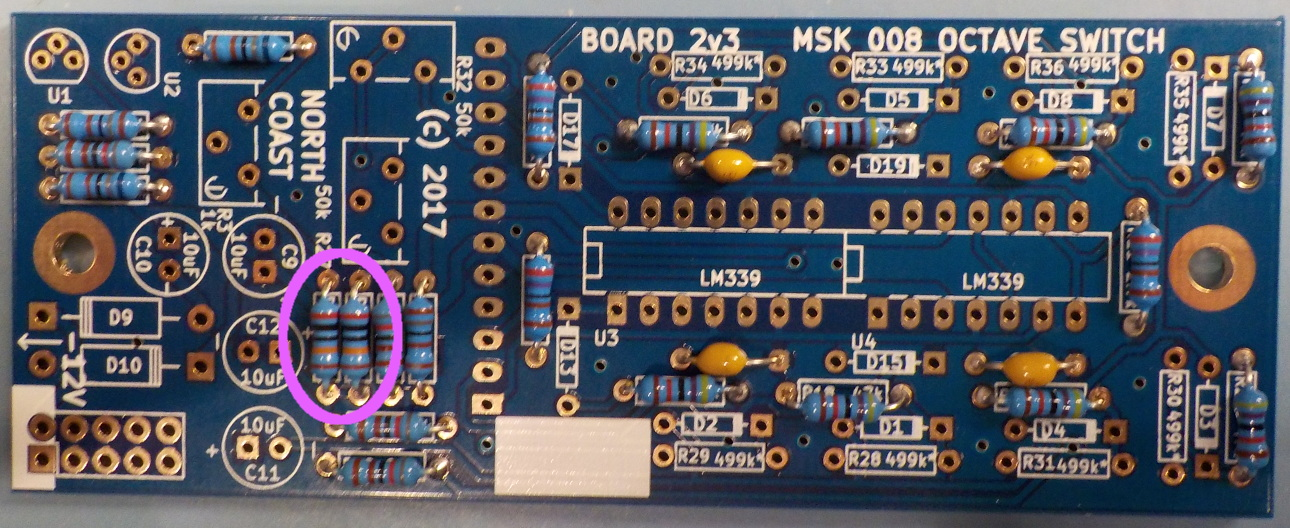
\includegraphics[width=\linewidth]{res-200k.jpg}

Install the eight 499k$\Omega$ 0.1\%\ (yellow-white-white-orange) precision
resistors R28 to R31 and R33 to R36.  These control the voltages of
individual steps in the quantizer outputs.  When building the prototypes I
noticed that either these resistors are just a little larger than others of
the same approximate body size, or maybe their leads are a little stiffer; I
found that I needed to bend the leads tighter (closer to the bodies) than
usual in order to have them fit nicely on the board.  Take it slowly and
carefully.

\noindent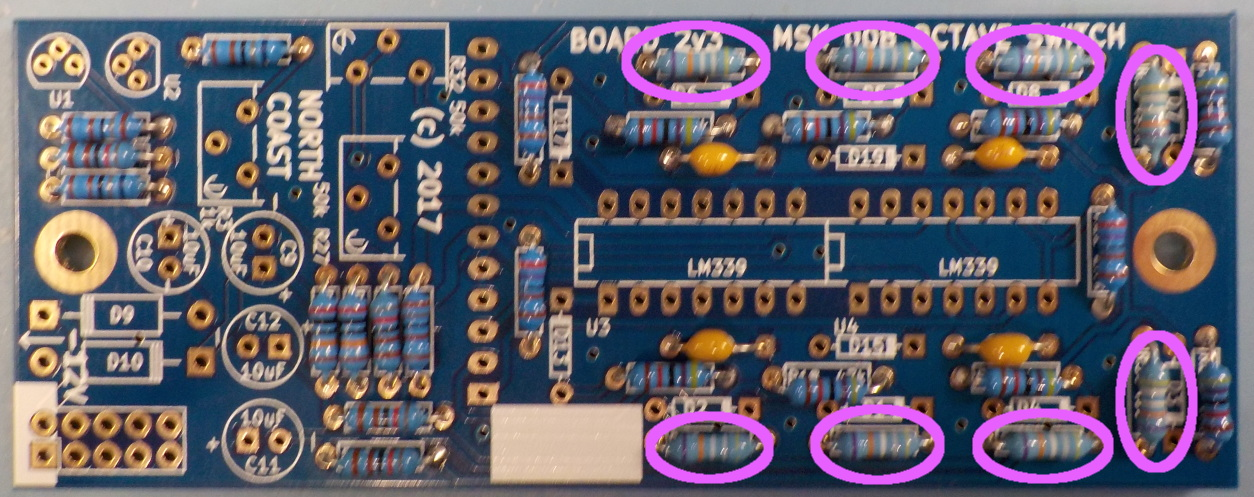
\includegraphics[width=\linewidth]{res-499k.jpg}

\section{Semiconductors}

Install the twelve 1N4148 or 1N914 switching diodes D1 to D8, D13, D15, D17,
and D19.  These act as switches to generate the proper output currents from
the quantizers.  They are polarized components and it is important to
install them right way round.  Each diode is packaged inside a pink glass
bead with a black stripe at one end; that end is the \emph{cathode}.  The
silkscreen markings on the board have a corresponding stripe and the diodes
should be installed with their stripes matching the markings on the board. 
The solder pads for the cathodes are also square instead of round. 
Installing one or more of these diodes backwards will result in incorrect
output voltages or input thresholds for the quantizers.

\noindent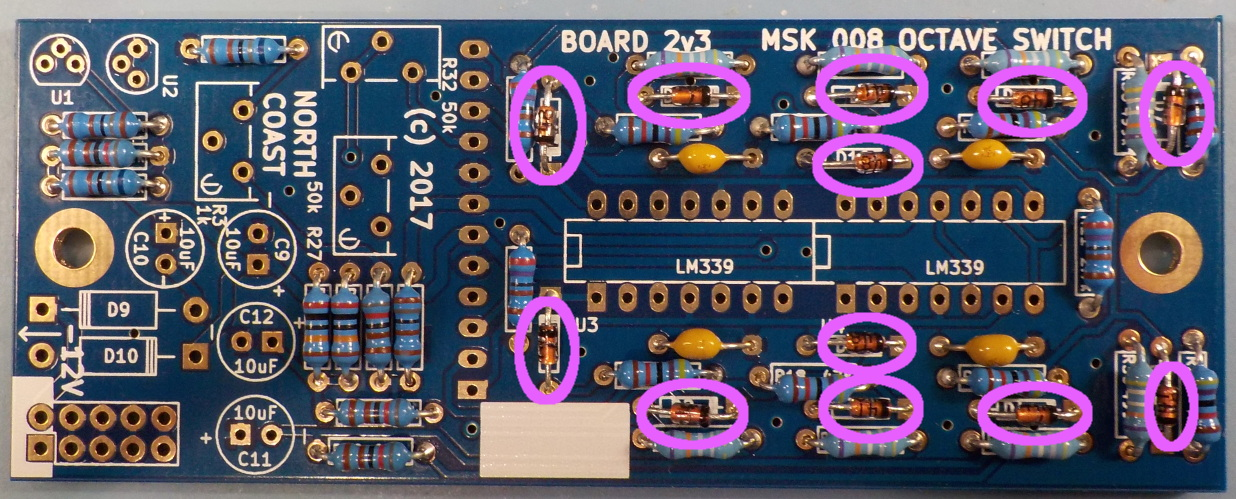
\includegraphics[width=\linewidth]{diodes2.jpg}

The switching diodes are the only small glass diodes in an MSK~008 kit, but
do not confuse them with other kinds of small glass diodes (such as Zeners)
that you might have on hand from other projects.  All diodes in this kind of
package look pretty much identical, distinguished only by their electrical
properties and near-microscopic code numbers etched onto the glass.

Note that a kit should include sixteen of these diodes, and only twelve are
used on this board; save the remaining four to install on Board~1.

Install the two 1N5818 or SBA130 Schottky rectifier diodes D9 and D10. 
These are for reverse-voltage protection; they cut off power to the module
when the power plug is backwards.  They are polarized and it is important to
install them in the right direction.  As with the switching diodes, these
diodes will be marked with stripes indicating their cathodes (here, probably
white or light grey paint on a black or dark grey plastic package) and those
stripes should match the stripes on the PCB silkscreen.  The cathode solder
pads are also square.  Installing these backwards means they will have the
opposite of the intended protective effect.

\noindent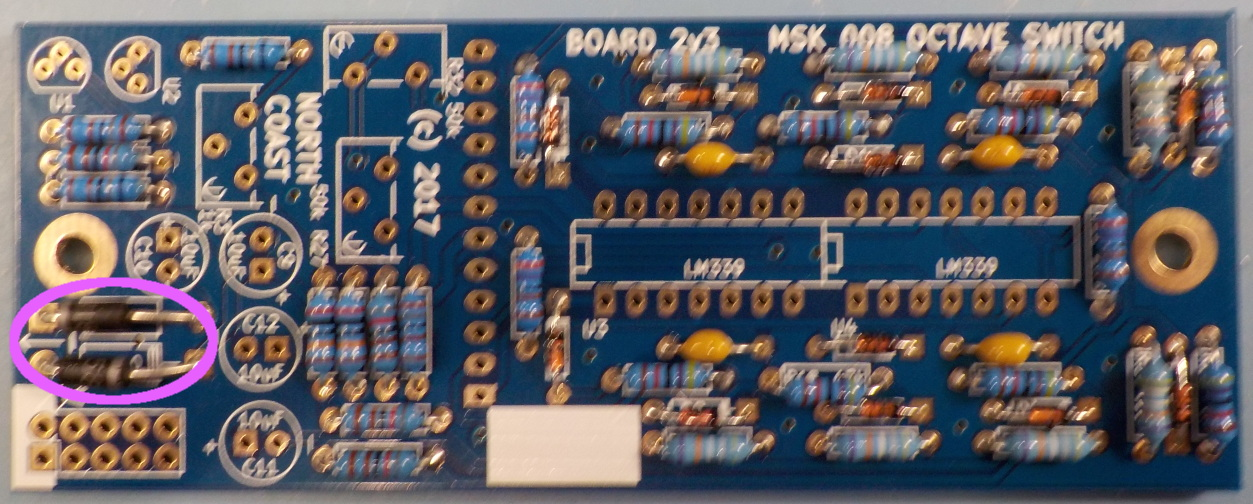
\includegraphics[width=\linewidth]{schottky.jpg}

Install the two 14-pin DIP sockets for the LM339 quad comparator chips, U3
and U4.  These chips test input voltages against reference values in the
quantizers.  The sockets themselves do not care which direction you install
them, but it is critically important that the chips installed in the sockets
should be installed in the right direction.  To help with that, the sockets
will probably be marked with notches at one end (indicating the end where
Pin~1 and Pin~14 are located) and you should install the sockets so that the
notched ends match the notches shown on the PCB silkscreen.  The solder pad
for Pin~1 is also distinguished by being rectangular instead of rounded.

Installing DIP sockets without having them tilted at a funny angle can be
tricky.  I recommend inserting the socket in the board, taping it in place
on the component side with vinyl electrical tape, then soldering one pin on
one corner and checking that the socket is snug against the board before
soldering the other pins.  That way, if you accidentally solder the first
pin with the socket tilted, it will be easier to correct (only one pin to
desolder instead of all of them).

\noindent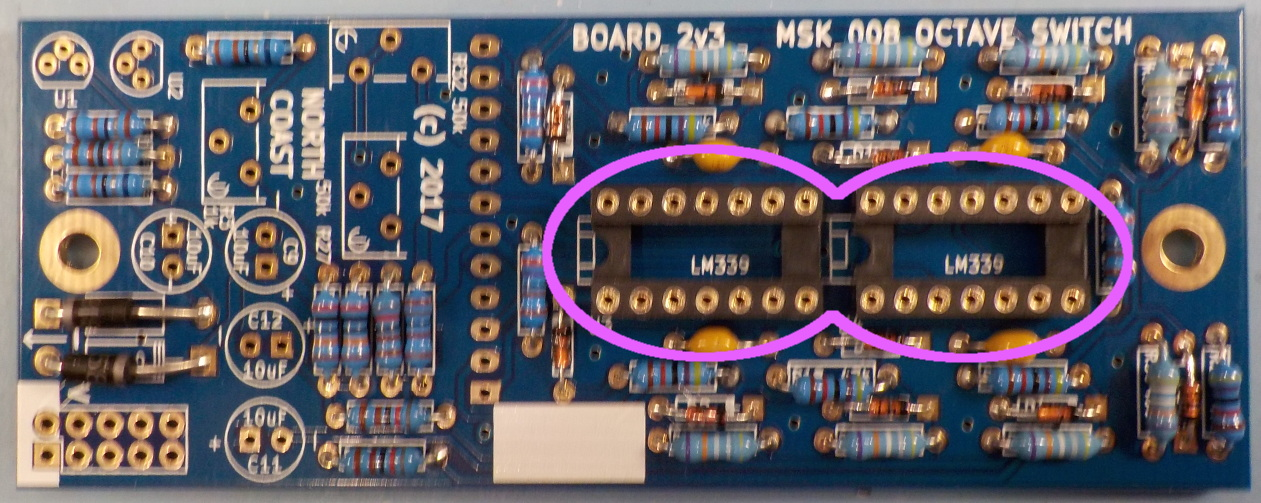
\includegraphics[width=\linewidth]{dip2.jpg}

If you somehow manage to solder an entire socket in backwards, don't try to
desolder it to turn it around.  Just leave it as it is and remember that
when you insert the chip, you must insert it so the chip matches the
markings on the \emph{board}, not the turned-around socket.

Install the two TL431 voltage regulator chips U1 and U2, which provide the
$\pm$4.5V reference voltages for the quantizer.  These are packaged
in epoxy plastic TO-92 pills like transistors, but they are actually
complete integrated circuits each comprising about ten transistors and some
other components.  They are polarized and will be destroyed if installed in
the wrong direction.  Each chip's place on the board is shown by a
silkscreened circle with one flattened side, and the chip packages are
similarly rounded with one flat side; install the chips so that their flat
sides match the ones shown on the board.  The middle one of the three legs
should be carefully bent backward to match the triangular arrangement of
holes on the board, and the body of the package should sit at least a few
millimetres above the board.  Push it down far enough for the legs to be
snug in the holes, but do not attempt to seat the package flush to
the board.

\pagebreak

Be aware that the solder holes for these chips are small and close together,
and be careful to avoid making solder bridges between them.

\noindent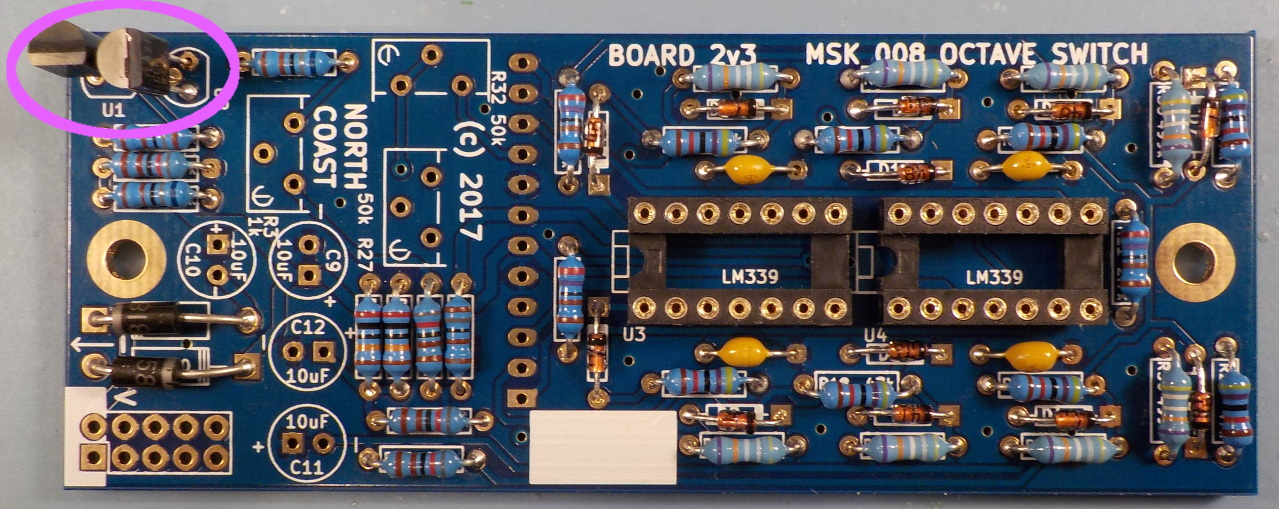
\includegraphics[width=\linewidth]{vreg.jpg}

\section{Board to board connectors}

Although the sequence is not critical, I recommend installing the male
header connector (P2) that links Board~2 to Board~1 at this time, before the
taller components like electrolytic capacitors and trimmers, because once
those are in place they may restrict access to the solder pads for the
header.  For best alignment, you should solder the male connector while it
is mated with the female connector (J9) on Board~1, and it's convenient to
solder the Board~1 connector at this time too.

Mate the two connectors firmly, then assemble the two boards and the
connectors using the M3 machine screws and 10mm and 11mm standoffs, as
shown.  The 11mm standoffs should separate the two boards; I suggest using
the 10mm standoffs instead of hex nuts for this temporary assembly because
they're easier to tighten by hand.  Do not confuse the two lengths.  Solder
the connectors on both boards.  Then disassemble them, and set aside the
hardware and Board~1 for later.

Note that the first batch of female header connectors I bought for this
project were an expensive low-profile type that I decided not to continue
using in the long term, because their main advantage would be allowing the
boards to fit closer together, and other components make it hard to take full
advantage of that.  If you have an early kit, you may have one of these
connectors, and they are the type shown in the photos.  The low-profile
female connectors, mated with the male headers, add up to slightly less than
11mm; so there will be a little bit of play in the temporary assembly, and
you should try to adjust the connector positions before soldering so that
both the male and female sides fit nicely in their corresponding holes in
the PCBs.  Later kits will have a taller female connector that fits the
design spacing more precisely.

\noindent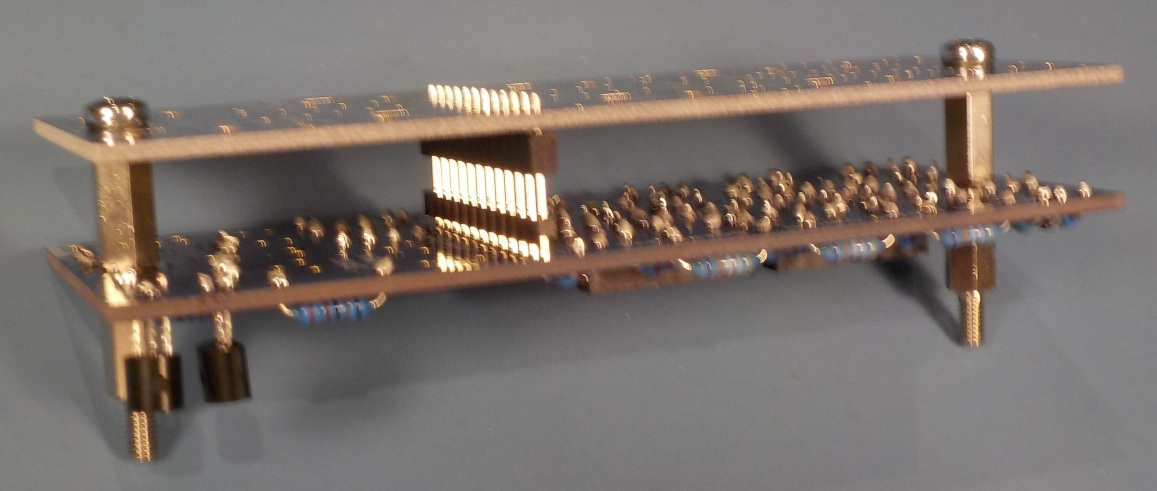
\includegraphics[width=\linewidth]{b2b-stack.jpg}

\section{Electrolytic capacitors}

Install the four 10$\mu$F electrolytic capacitors C1 through C4, which
filter the power supply and reference bussesfor the module as a whole. 
These are polarized components and they may explode if installed backwards. 
Each one will be marked on its casing with a stripe and minus signs to
indicate the negative lead; the positive lead will probably also be longer. 
These clues should be matched with the markings on the PCB: plus and minus
symbols in the silkscreen and a square solder pad for the positive (long)
lead.

\noindent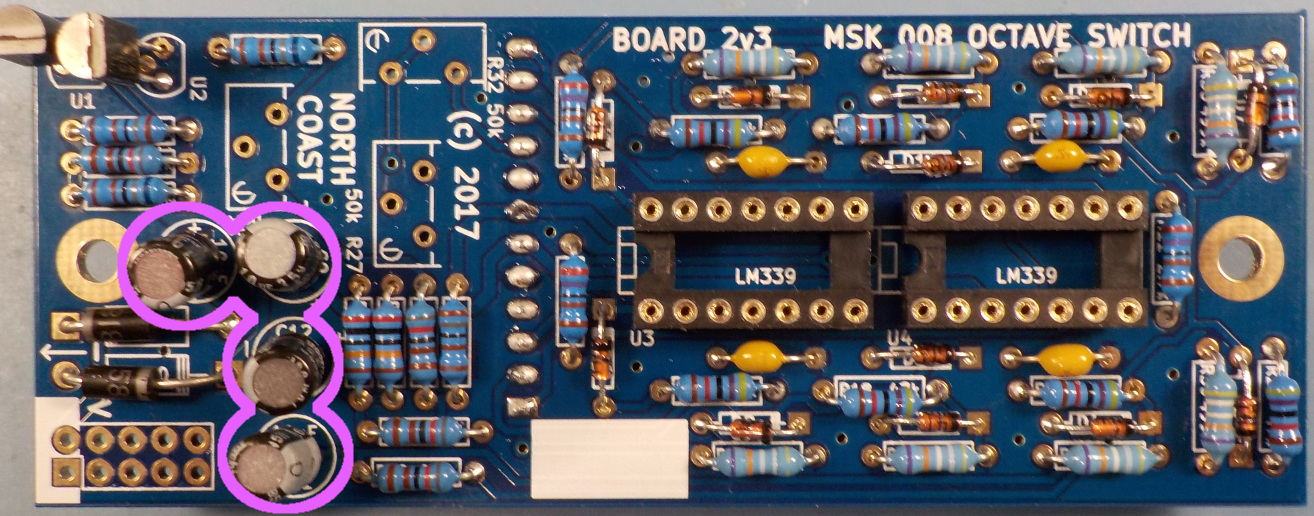
\includegraphics[width=\linewidth]{cap-10u.jpg}

\section{Trimmer potentiometers}

If you have not already set the trimmers to 50\%\ of their full scale value
as described under ``Preliminaries'' above, then do it now.  Also, take note
of the comments about incorrectly-labelled trimmers in that section.

Trimmers usually are not washable, so if you plan to clean your boards by
full immersion in water or other solvent,\footnote{Did you hear the one
about the hipster who was told to clean circuit boards with ``IPA,'' and
used India Pale Ale?} your last chance is now; future cleaning will have to
be done with a brush and some care to avoid letting liquid seep into the
trimmers.  Even now you should take some care with the DIP sockets, because
solvent can carry flux residue into them and form a varnish-like layer if
not carefully rinsed away.

Trimmers are not exactly polarized, but the three legs of each trimmer serve
different functions and need to be connected to the right holes.  The
physical arrangement of the legs and corresponding holes should make it
impossible to install the trimmers wrong way round.

Install the 1k$\Omega$ trimmer R3.  This trimmer's main purpose is to adjust
the higher-voltage output levels of both quantizer channels.  What it
directly controls is the voltage on the -4.5V reference bus.

\noindent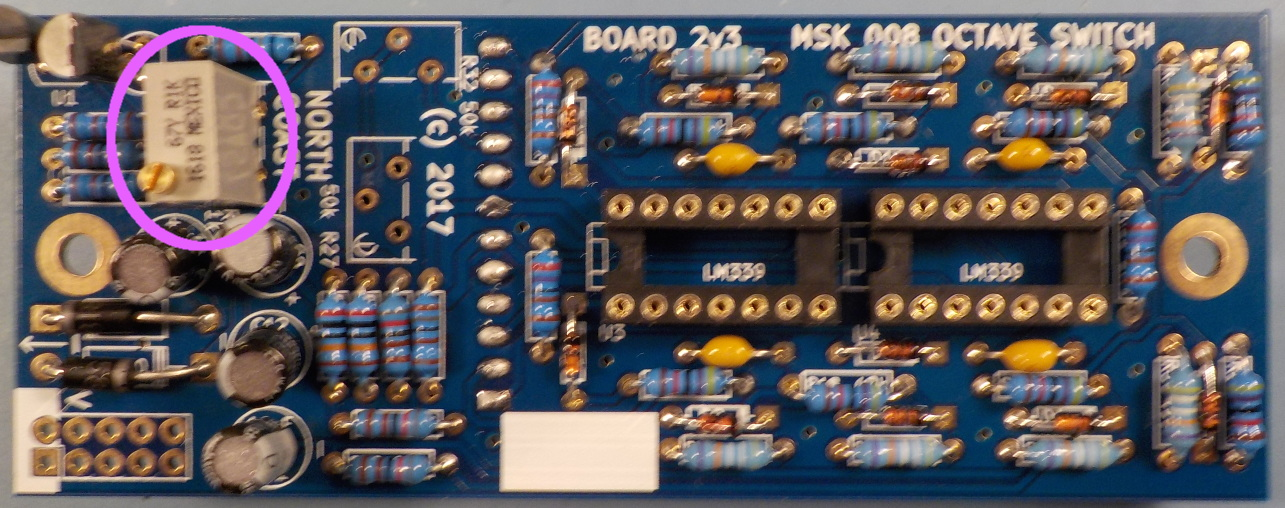
\includegraphics[width=\linewidth]{pot-1k.jpg}

Install the two 50k$\Omega$ trimmers R27 and R32.  These trimmers adjust the
lower-voltage output levels of the quantizers, one trimmer for each channel. 
Their direct function is to control the offsetting current fed into the
final summing amplifiers.

\noindent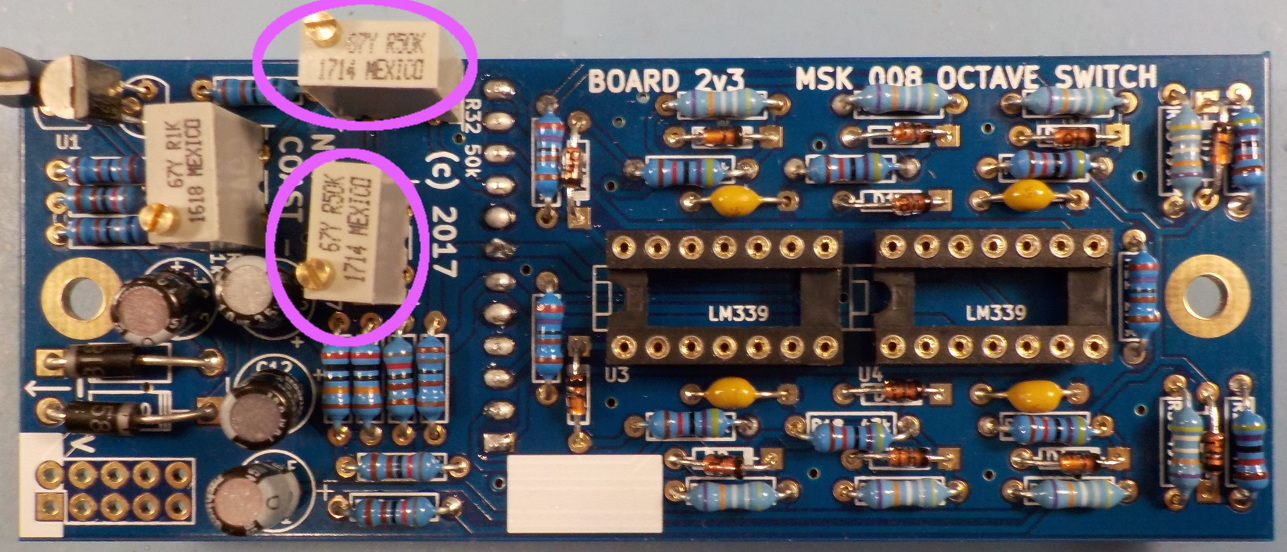
\includegraphics[width=\linewidth]{pot-50k.jpg}

\section{Eurorack power connector}

Install the 2$\times$5-pin Eurorack power connector.  This connector is not
polarized in itself, although the connection it makes is polarized.  As with
the DIP sockets, you should be careful to get it installed snugly against
the board, not tilted at an angle.  Use vinyl tape or similar to hold it in
place, solder one pin, then check that it is straight before you solder the
other pins.

Be aware that both the connector and the copper connections to it on the PCB
have relatively large thermal mass.  These solder joints will need more
heat than usual; and after you have soldered it, the connector will remain
hot longer than recently-soldered components usually do.  Don't burn
yourself.

The six pins in the centre of the connector, that is all except the four
corner pins, are for grounding and they are all connected together on the
board.  Thus, if you accidentally form solder bridges among these six pins
while installing the connector, don't waste effort trying to remove them;
they will have no electrical effect.

\noindent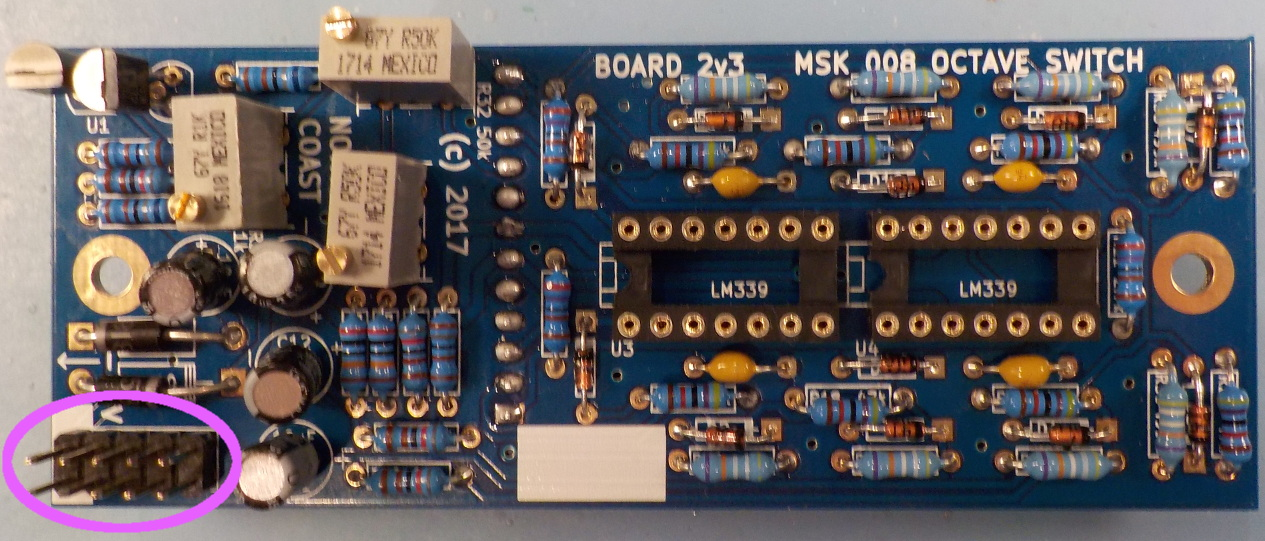
\includegraphics[width=\linewidth]{power.jpg}

In between completed boards is a good time to take a break.
